\documentclass[handout]{beamer}

\usepackage{Vor2018glærur}

\title{Tölvunarfræði 2}
\subtitle{Vika 6}

\begin{document}

\begin{frame}
\titlepage
\end{frame}

\section{Inngangur}

\begin{frame}{Af hverju röðun?}
\begin{itemize}
 \item Skoðum röðun í dag!
 \item Röðun er vel leyst vandamál - af hverju skoðum við þetta svona vel?
 \begin{itemize}
  \item Röðunarreiknirit eru oft auðgreinanleg - góð æfing
  \item Forritunarmynstur sem koma upp við röðun birtast oft í öðrum samhengjum
  \item Röðunarreiknirit koma við sögu sem hluti af stærri reikniritum
 \end{itemize}
\end{itemize}
\end{frame}

\section{Comparable og uppbygging röðunarklasa}

\begin{frame}{Comparable skilin}
\begin{itemize}
 \item Hverju er hægt að raða?
 \item Munum skoða röðunaraðferðir sem byggjast á samanburðum
 \begin{itemize}
  \item Til að skilgreina hluti sem samanberanlega í Java getum við látið viðkomandi klasa uppfylla \href{https://docs.oracle.com/javase/8/docs/api/java/lang/Comparable.html}{Comparable skilin}
  \item Ein aðferð - \texttt{compareTo}
 \end{itemize}
\end{itemize}
\end{frame}


\begin{frame}{Kröfur \texttt{compareTo}}
\begin{itemize}
 \item \texttt{a.compareTo(b)} skilar eftirfarandi:
 \begin{itemize}
  \item Neikvæðri tölu ef $a < b$
  \item 0 ef $a = b$
  \item Jákvæðri tölu ef $a > b$
 \end{itemize}

 \item Nokkrar kröfur eru áskildar í aðferðinni
 \begin{itemize}
  \item \texttt{x.compareTo(y)} og \texttt{y.compareTo(x)} hafa gagnstæð formerki eða eru bæði 0
  \item Ef \texttt{x.compareTo(y)>0 \&\& y.compareTo(z)>0} þá \texttt{x.compareTo(z)>0}
  \item Ef \texttt{x.compareTo(y)==0} þá hafa \texttt{x.compareTo(z)} og \texttt{y.compareTo(z)} sama formerki
 \end{itemize}
\end{itemize}
\end{frame}

\begin{frame}{Uppbygging röðunarklasa}
\begin{itemize}
 \item Við munum forrita á móti Comparable skilunum
 \begin{itemize}
  \item Í stað þess að gera ráð fyrir að hluturinn sem unnið er með sé tilvik af ákveðnum klasa, þá gerum við ráð fyrir að hluturinn uppfylli ákveðin skil
  \item Notum nafnið á skilunum eins og þau væru nafn á gagnagerð 
  \item Gerir klasana sveigjanlegri
 \end{itemize}
\end{itemize}
\end{frame}

\begin{frame}{Dæmi um klasa}
\javafile[firstline=10, lastline=23, fontsize=\scriptsize, label=Example.java]{Code/w6/Example.java}

(Algorithms bls. 245)
\end{frame}

\section{Eiginleikar röðunarreiknirita}

\begin{frame}{Eiginleikar röðunarreiknirita}
\begin{itemize}
 \item Mörg mismunandi röðunarreiknirit eru til, getum metið þau m.t.t. mismunandi eiginleika
 \begin{itemize}
  \item Keyrslutími
  \begin{itemize}
   \item Teljum fjölda samanburða, víxlana (e. \emph{swaps}) og eða fylkjaaðgerðir sem fall af inntaksstærð
  \end{itemize}
  \item Minniskrafa
  \begin{itemize}
   \item Þurfum við að geyma afrit af safninu sem við erum að raða?
  \end{itemize}
  \item Hversu almennt er það?
  \begin{itemize}
   \item Okkar röðunarreiknirit virka á gögn sem uppfylla \texttt{Comparable}
   \item Aðrir möguleikar eru til (sjá: Radix Sort, Counting Sort)
  \end{itemize}
  \item Er það stöðugt \eng{stable}?
 \end{itemize}
\end{itemize}
\end{frame}

\section{Nokkur röðunarreiknirit}

\begin{frame}{Valröðun}
\begin{itemize}
 \item Valröðun \eng{selection sort} er einfaldasta röðunnarreikniritið okkar
 \item Lýsing:
 \begin{enumerate}
  \item Finnum minnsta stakið í safninu, setjum það fremst
  \item Finnum næstminnsta stakið í safninu, setjum það næstfremst
  \item Höldum áfram þar til safninu er raðað
 \end{enumerate}
 \item Þarf $\sim \frac{N^2}{2}$ samanburði og $N$ víxlanir
 \begin{itemize}
  \item Margir samanburðir, lágmarksfjöldi víxlana
 \end{itemize}
 \item Skoðum Selection.java 
\end{itemize}
\end{frame}

\begin{frame}{Innsetningarröðun}
\begin{itemize}
 \item Innsetningarröðun \eng{insertion sort} er aðferð sem er lík þeirri sem fólk notar venjulega við að raða raunverulegum hlutum
 \item Lýsing:
 \begin{enumerate}
  \item Höldum utan um ``raðaðan hluta'' til vinstri og ``óraðaðan hluta'' til hægri í safninu
  \item Tökum það stak sem lengst er til vinstri í óraðaða hlutanum
  \item Færum það lengra til vinstri þar til við rekumst á minna stak
  \item Færum mörk undirsafnanna eitt stak til hægri og endurtökum
 \end{enumerate}
 \item Mismunandi keyrslutími eftir tilvikum:
 \begin{itemize}
  \item $\sim \frac{N^2}{2}$ samanburðir og $\sim \frac{N^2}{2}$ víxlanir í versta tilvikinu
  \item $\sim \frac{N^2}{4}$ samanburðir og $\sim \frac{N^2}{4}$ víxlanir ``að meðaltali''
  \item $n-1$ samanburðir og engar víxlanir í besta tilvikinu 
 \end{itemize}
 \item Skoðum Insertion.java
\end{itemize}
\end{frame}

\begin{frame}{Sameiningarröðun}
\begin{itemize}
 \item Sameiningarröðun \eng{merge sort} er skilvirk röðunaraðferð fyrir stóra lista
 \item Lýsing:
 \begin{itemize}
  \item Skilgreinum uppskiptingu á safninu svo úr verði hlutsafn
  \item Skilgreinum uppskiptingar á sama hátt þar til hlutsöfnin eru af viðráðanlegri stærð
  \item Sameinum hlutsöfnin svo úr verði raðað hlutsafn
 \end{itemize}
 \item Þarf milli $\frac{N \log N}{2}$ og $N \log N$ samanburði, $\sim 6N\log N$ fylkjaaðgerðir
 \begin{itemize}
  \item Gott, en við þurfum auka minni!
 \end{itemize}
 \item Skoðum Merge.java
 \begin{itemize}
  \item Hér er ofansækinni \eng{top-down} sameiningarröðun lýst
 \end{itemize}
\end{itemize}
\end{frame}

\begin{frame}{Skema}
\begin{center}
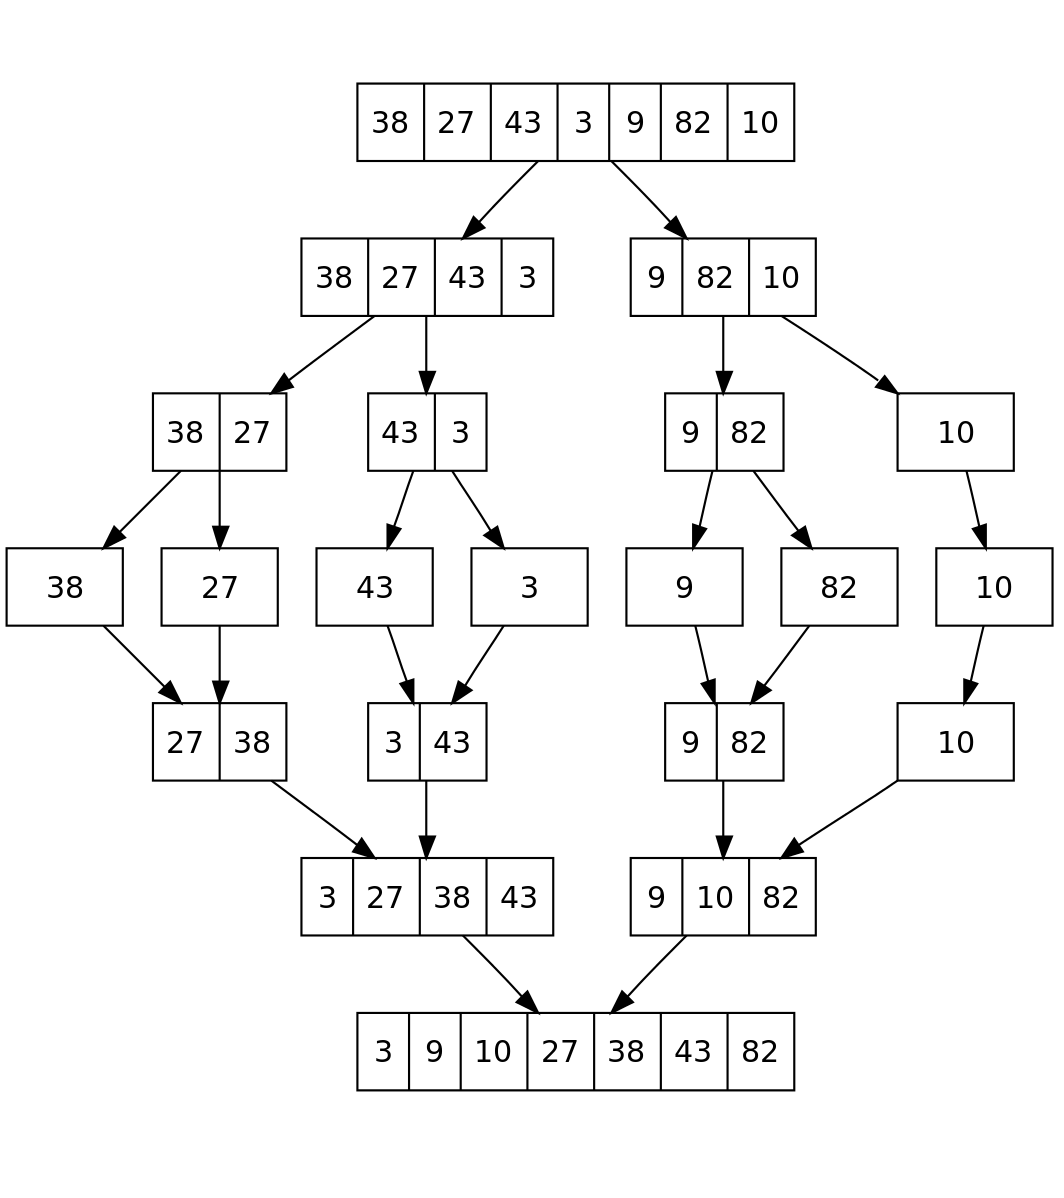
\includegraphics[width=0.7\textwidth]{merge-sort-diagram}
\end{center}
\end{frame}


\begin{frame}{Trix}
\begin{itemize}
 \item Notum innsetningarröðun á lítil söfn eða þegar þau eru nær röðuð
 \begin{itemize}
  \item Algengt að raunveruleg forritunarmál noti þessa aðferð
  \item \href{https://docs.oracle.com/javase/8/docs/api/java/util/Arrays.html}{sort} í Java 8
 \end{itemize}
 \item Neðansækin \eng{bottom-up} sameiningarröðun er meira viðeigandi fyrir eintengda lista
 \begin{itemize}
  \item Brjóta vandamálið niður og leysa hlutana endurkvæmt - ofansækin aðferð
  \item Leysa lítil vandamál sem sameinast í stærri lausn - neðansækin aðferð
 \end{itemize}
\end{itemize}
\end{frame}

\section{Lokaorð}

\begin{frame}{Tenglar}
\begin{itemize}
 \item \href{https://www.toptal.com/developers/sorting-algorithms/}{Einföld yfirlitssíða}
 \begin{itemize}
  \item Varúð - síðan hefur eitthvað að selja
 \end{itemize}
 \item \href{https://www.youtube.com/watch?v=kPRA0W1kECg}{The Sound of Sorting}
 \begin{itemize}
  \item Varúð - hljóð
 \end{itemize}
 \item \href{https://www.youtube.com/watch?v=ROalU379l3U}{Röðunardans}
 \begin{itemize}
  \item Varúð - dansandi fólk
 \end{itemize}
 \item \href{https://www.youtube.com/watch?v=es2T6KY45cA}{Vélmenni raða}
\end{itemize}
\end{frame}


\begin{frame}{Þessi glærupakki}
Tengill á fyrirlestraræfingu: \url{https://goo.gl/forms/xRQCjHXFQ82B56yf2}
\vspace{1cm}

Example.java má finna á \href{https://github.com/Ernir/kennsluefni/tree/master/T2/Code/w6}{Github}. 

Kóða fyrir röðunarreikniritin má finna á \url{http://algs4.cs.princeton.edu/code/}
\end{frame}

\begin{frame}{Næst}
Quicksort reikniritið, forgangsbiðraðir, miðmisseriskönnun
\end{frame}


\end{document}
